\documentclass[tikz]{standalone}
\usepackage{pgfplots}
\pgfplotsset{compat=1.18}
\begin{document}
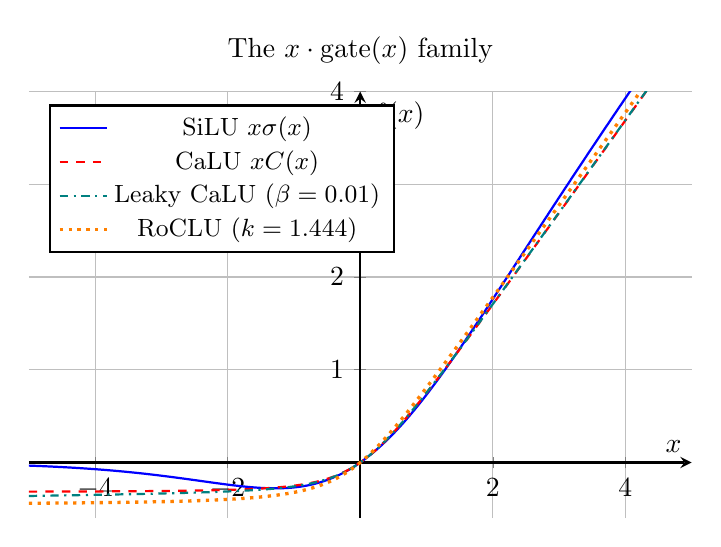
\begin{tikzpicture}
\begin{axis}[
  width=10cm, height=7cm,
  xlabel=$x$, ylabel=$f(x)$,
  title={The $x \cdot \mathrm{gate}(x)$ family},
  xmin=-5, xmax=5, ymin=-0.6, ymax=4,
  axis x line=middle, axis y line=middle,
  grid=major, legend pos=north west,
  legend style={font=\small},
  samples=300, thick,
]
\addplot[blue] {x/(1+exp(-x))};
\addlegendentry{SiLU $x\sigma(x)$}
\addplot[red, dashed] {x*(0.5 + atan(x)/180)};
\addlegendentry{CaLU $xC(x)$}
\addplot[teal, dashdotted] {0.99*x*(0.5 + atan(x)/180) + 0.01*x};
\addlegendentry{Leaky CaLU ($\beta=0.01$)}
\addplot[orange, dotted, very thick] {x*1.444*ln(1.5 + atan(x)/180)};
\addlegendentry{RoCLU ($k=1.444$)}
\end{axis}
\end{tikzpicture}
\end{document}
